\documentclass{beamer}

% Must be loaded first
\usepackage{tikz}

\usepackage[utf8]{inputenc}
\usepackage{textpos}

% Font configuration
\usepackage{fontspec}

\input{font.tex}

% Tikz for beautiful drawings
\usetikzlibrary{mindmap,backgrounds}
\usetikzlibrary{arrows.meta,arrows}
\usetikzlibrary{shapes.geometric}

% Minted configuration for source code highlighting
\usepackage{minted}
\setminted{highlightcolor=black!5, linenos}
\setminted{style=perldoc}

\usepackage[listings, minted]{tcolorbox}
\tcbset{left=6mm}

% Use the include theme
\usetheme{codecentric}

% Metadata
\title{How This Presentation Was Made}
\author{Markus Hauck @markus1189}

\newcommand{\overview}{%
    \begin{center}
  \resizebox{0.7\textwidth}{!}{
  \begin{tikzpicture}
  \path[small mindmap, concept color=beamer@codeblue,
  level 1 concept/.append style={every child/.style={concept color=beamer@centricgreen}},
  level 2 concept/.append style={every child/.style={concept color=beamer@centricgreen!50}}
  ]
  node[concept] {Presentation}
  [clockwise from=0]
  child {
    node[concept] (images) {Images}
    [clockwise from=90]
    child { node[concept] (algo) {Download} }
    child { node[concept] {graphviz} }
    child { node[concept] {ditaa} }
    child { node[concept] {plantuml} }
  }
  child {
    node[concept] (code) {Code}
    [clockwise from=-90]
    child { node[concept] {Extract} }
    child { node[concept] {Inline} }
  }
  child {
    node[concept] (build) {Build}
    [clockwise from=-120]
    child { node[concept] {PDF} }
    child { node[concept] {Depen-\\dencies} }
    child { node[concept] {CI} }
  }
  child {
    node[concept] (tools) {Tools}
    [clockwise from=135]
    child { node[concept] {Dhall} }
    child { node[concept] {Shake} }
    child { node[concept] {Nix} }
  }

  node [annotation, xshift=2cm, yshift=-10mm] (annot) at (code.east) {
    \setsansfont{Caveat} \large Should compile }
  node [annotation, xshift=2cm, yshift=-10mm] (annot2) at (build.east) {
    \setsansfont{Caveat} \large Simple }
  node [annotation, xshift=-10mm, yshift=8mm] (annot3) at (images.north) {
    \setsansfont{Caveat} \large Generated}
  node [annotation] (annot4) at (tools.west) { % TODO
    \setsansfont{Caveat} \large Fun}
  ;

  \begin{pgfonlayer}{background}
    \draw[draw=black, thick, shorten <=1mm, shorten >=1mm, -{Stealth[length=3mm, open, round]}] (annot) edge (code);
    \draw[draw=black, thick, shorten <=1mm, shorten >=1mm, -{Stealth[length=3mm, open, round]}] (annot2) edge (build);
    \draw[draw=black, thick, shorten <=1mm, shorten >=1mm, -{Stealth[length=3mm, open, round]}] (annot3) edge (images);
    \draw[draw=black, thick, shorten <=1mm, shorten >=1mm, -{Stealth[length=3mm, open, round]}] (annot4) edge (tools);
  \end{pgfonlayer}
\end{tikzpicture}
}
  \end{center}
}

% The presentation content
\begin{document}

\begin{frame}[noframenumbering,plain]
  \titlepage{}
\end{frame}

\section{Introduction}\label{sec:introduction}

\begin{frame}
  \frametitle{Presentations}
  \begin{center}
    \includegraphics[width=\textwidth]{ditaa/presentations.png}
  \end{center}
\end{frame}

\begin{frame}
  \frametitle{Some Problems}
  \begin{itemize}
  \item powerpoint/keynote/google slides/\ldots{}
  \item but you can't use \texttt{git}
  \item pandoc / LaTeX / \ldots{}
  \item how to include code and pictures?
  \end{itemize}
\end{frame}

\begin{frame}
  \frametitle{How It All Started}
  \begin{itemize}
  \item Me writing presentation be like:
  \item fighting graphical editor more than focused on content
  \item logical step: switch to something that is text based
  \item how to handle generated pictures
  \item how to handle code
  \end{itemize}
\end{frame}

\begin{frame}
  \frametitle{Used Tools Overview}
  \begin{itemize}
  \item Nix for system dependencies + build env
  \item Shake to write a custom build system
  \item Dhall for ``configuration''
  \item LaTeX for slides
  \item ditaa, graphviz
  \end{itemize}
\end{frame}

\begin{frame}
  \frametitle{Wish List}
  \begin{itemize}
  \item version control: use git to track changes
  \item reproducible: same description for CI and local machine
  \item single step: \textbf{one} command to build presentation
  \item declarative: generate from description
  \item checked: source code compiles
  \item minimal: only re-build what changed
  \end{itemize}
\end{frame}

\begin{frame}
  \frametitle{Overview}
  \overview{}
\end{frame}

\section{Shake}

\begin{frame}
  \frametitle{Tool: Shake}
  \begin{itemize}
  \item \url{shakebuild.com/manual}
  \item Shake is a Haskell \textbf{library} for writing build systems
  \item ``just'' a library, rest is up to you
  \item \texttt{Shake} vs \texttt{make} is like \texttt{Monad} vs \texttt{Applicative}
  \item integrates well with other libraries and system tools
  \end{itemize}
\end{frame}

\begin{frame}
  \frametitle{Shake \textemdash{} Usage}
  \begin{itemize}
  \item specify rules to create output from some input
  \item avoid rebuilds of unchanged things
  \item call the shake build from your \texttt{main}
  \end{itemize}
\end{frame}

\begin{frame}[fragile]
  \frametitle{Shake Rules}
  \begin{minted}{haskell}
--  +---------------- file pattern to match
--  |
--  |       +-------- target path to create
--  |       |
--  v       v
pattern %> \out -> do
  action1          -- <--\
  action2          -- <---+- Actions to build 'out'
  action3          -- <--/
  \end{minted}
\end{frame}

\begin{frame}[fragile]
  \frametitle{Shake Rules}
  \begin{minted}{haskell}
"*.txt" %> \out -> do
  putNormal "Debug"
  cmd "touch" [out]
  \end{minted}
\end{frame}

\begin{frame}[fragile]
  \frametitle{Shake Rules}
  \inputminted[autogobble]{haskell}{snippets/pdf-rule.hs}
  \inputminted[autogobble]{haskell}{snippets/latexmk-rule.hs}
\end{frame}

\begin{frame}
  \frametitle{Shake Rules}
  \begin{center}
    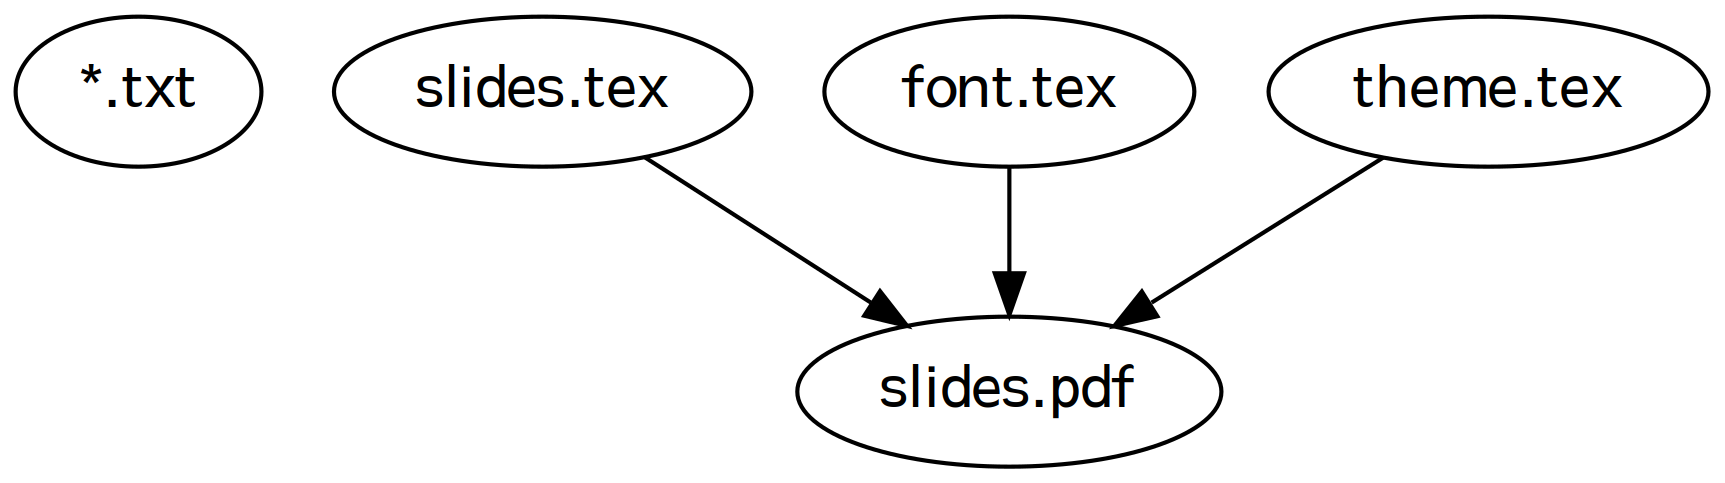
\includegraphics[width=0.8\textwidth]{graphviz/rules.png}
  \end{center}
\end{frame}

\begin{frame}
  \frametitle{Shake}
  \begin{itemize}
  \item general idea: express any dependencies via Shake rules
  \item let shake figure out what needs rebuilding
  \item next up: source code
  \end{itemize}
\end{frame}

\section{Source Code}

\begin{frame}
  \frametitle{Editing Code}
  \begin{itemize}
  \item Step 1: Implement your code in a normal project
  \item Step 2: Wild Copy And Paste Into Presentation
  \item Step 3: Reformat To Fit Slide
  \item Step 4: Change Original Source Code
  \item Step 5: Wild Editing Of Code on Slides
  \item Step 6: Notice something doesn't make sense
  \end{itemize}
\end{frame}

\begin{frame}[fragile]
  \frametitle{Extract Code}
  \begin{itemize}
  \item totally broken: copy \& paste
  \item little better: extract based on lines
  \item after edit / formatting / \ldots they change
  \item not what we want
  \end{itemize}
\end{frame}

\begin{frame}
  \frametitle{Editing Code}
  \begin{itemize}
  \item idea: extract source code directly from actual project
  \item use comments to delimit ``snippets''
  \item write code to extract everything in between
  \end{itemize}
\end{frame}

\begin{frame}
  \frametitle{Editing Code}
  \begin{itemize}
  \item add comments in the code
  \item write a small ``snippet'' file
  \item let shake automatically extract snippets
  \item include code snippets in presentation
  \end{itemize}
\end{frame}

\begin{frame}
  \frametitle{Annotating Code for Snippets (META)}
  \begin{center}
    \inputminted[autogobble]{haskell}{snippets/outer-pdf-rule.hs}
  \end{center}
\end{frame}

\begin{frame}
  \frametitle{Intermezzo: Dhall}
  \begin{quote}
    A configuration language guaranteed to terminate
  \end{quote}
  \begin{itemize}
  \item think: lambda calculus for config
  \item not turing-complete on purpose
  \item subset can be converted to JSON and YAML
  \item can be mapped directly into Haskell types
  \end{itemize}
\end{frame}

\begin{frame}
  \frametitle{Dhall Example}
  \inputminted[autogobble]{haskell}{dhall/example.dhall}
\end{frame}

\begin{frame}
  \frametitle{Dhall Features}
  \begin{itemize}
  \item booleans/integer/naturals
  \item optional values
  \item lists
  \item records
  \item functions
  \item strings + interpolation
  \item unions
  \item imports
  \item \ldots{}
  \end{itemize}
\end{frame}

\begin{frame}
  \frametitle{Dhall To JSON}
  \inputminted[autogobble]{json}{dhall/example.json}
\end{frame}

\begin{frame}
  \frametitle{Dhall To YAML}
  \inputminted[autogobble]{yaml}{dhall/example.yaml}
\end{frame}

\begin{frame}
  \frametitle{Snippet Files \textemdash{} Type}
  \begin{center}
    \inputminted{text}{snippets/snippet-type.dhall}
  \end{center}
\end{frame}

\begin{frame}
  \frametitle{Snippet Files \textemdash{} Example}
  \begin{center}
    \inputminted{text}{snippets/snippet-type.snippet}
  \end{center}
\end{frame}

\begin{frame}
  \frametitle{Snippet Files \textemdash{} Example}
  \begin{center}
    \inputminted{text}{snippets/pdf-rule.snippet}
  \end{center}
\end{frame}

\begin{frame}
  \frametitle{Snippet Rule \textemdash{} Broken Formatting}
  \begin{center}
    \inputminted[autogobble, highlightlines={3}]{haskell}{snippets/outer-haskell-snippet-rule.hs_noformat}
  \end{center}
\end{frame}

\begin{frame}
  \frametitle{Snippet Rule \textemdash{} After Auto-Formatting}
  \begin{center}
    \inputminted[autogobble, highlightlines={2-4}]{haskell}{snippets/haskell-snippet-rule.hs}
  \end{center}
\end{frame}

\begin{frame}
  \frametitle{Extracting Code}
  \begin{itemize}
  \item will always be up to date with the compiling source (yay)
  \item but we also have to format and maybe check again
  \end{itemize}
\end{frame}

\begin{frame}
  \frametitle{Checking Code}
  \begin{itemize}
  \item let's tackle checking first
  \item lots of times: broken code snippets that don't compile
  \item style errors you would notice in your actual setup
  \item after extracting a snippet into an includable file
  \item run linter/compiler/\ldots
  \item fail building presentation if the command fails
  \end{itemize}
\end{frame}

\begin{frame}
  \frametitle{Checking Code}
  \begin{itemize}
  \item haskell with hindent + hlint
  \item scala with sbt and scalafmt
  \item actually any programming language and linter
  \end{itemize}
\end{frame}

\begin{frame}
  \frametitle{Formatting Code}
  \begin{itemize}
  \item just another step like linting
  \item run formatter of choice on the source file
  \item e.g.\ format to a width of 55 chars
  \end{itemize}
\end{frame}

\begin{frame}
  \frametitle{Formatting Code}
  \begin{itemize}
  \item example of code:
  \end{itemize}
\end{frame}

\section{Pictures}

\begin{frame}
  \frametitle{Pictures}
  \begin{itemize}
  \item scenario 1: search on the web and download
    \begin{itemize}
    \item but you will forget from where
    \item resize and rotate are manual steps
    \item you have to store them in git
    \end{itemize}
  \item scenario 2: generated from description
    \begin{itemize}
    \item graphviz graphs
    \item ditaa diagrams
    \item plantuml diagrams
    \item and more\ldots{}
    \end{itemize}
  \end{itemize}
\end{frame}

\begin{frame}
  \frametitle{Downloading Pictures}
  \begin{itemize}
  \item use Haskell and Shake to download on demand
  \item download of the file from the internet
  \item file that describes from where plus transformations
  \item transformations performed by imagemagick
  \end{itemize}
\end{frame}

\begin{frame}
  \frametitle{Downloading Pictures}
  \begin{center}
    \includegraphics{images/maintain-make.jpg}
  \end{center}
\end{frame}

\begin{frame}
  \frametitle{Downloading Pictures}
    \begin{center}
    \inputminted{text}{images/maintain-make.src}
  \end{center}
\end{frame}

\begin{frame}
  \frametitle{Downloading Pictures}
    \begin{center}
    \inputminted{haskell}{snippets/download-images.hs}
  \end{center}
\end{frame}

\begin{frame}
  \frametitle{Generating Pictures}
  \begin{itemize}
  \item second scenario: picture is generated
  \item there is a file that describes it + tool to render
  \item Steps:
    \begin{itemize}
    \item write the description file
    \item generate graphic
    \item include in presentation
    \item change description
    \item generate graphic
    \item include in presentation
    \item change description again\ldots{}
    \end{itemize}
  \end{itemize}
\end{frame}

\begin{frame}
  \frametitle{Shake It}
  \begin{itemize}
  \item express the dependency as a shake rule
  \end{itemize}
  \inputminted{haskell}{snippets/graphviz-rule.hs}
\end{frame}

\begin{frame}
  \frametitle{Everything As A Rule}
  \begin{center}
    \includegraphics[width=\textwidth]{graphviz/rules-big.png}
  \end{center}
\end{frame}

\begin{frame}
  \frametitle{Getting Dependencies}
  \begin{itemize}
  \item the missing piece: how to ``discover'' dependencies?
  \item all of hackage is available
  \item parse LaTeX via HaTeX (this time)
  \item use the pandoc library
  \item \ldots whatever you need
  \end{itemize}
\end{frame}

\section{Continuous Integration}

\begin{frame}
  \frametitle{Develop Environment}
  \begin{itemize}
  \item we freely mixed stuff and used lots of tools
    \begin{itemize}
    \item haskell + libraries
    \item imagemagick
    \item graphviz
    \item ditaa
    \item LaTeX plus packages and special font
    \item scala, sbt, scalafmt
    \end{itemize}
  \end{itemize}
\end{frame}

\begin{frame}
  \frametitle{Continuous Integration via Travis}
  \inputminted[linenos=false, fontsize=\tiny, lastline=31]{yaml}{static-source/long-travis-ci.yml}
\end{frame}

\begin{frame}
  \frametitle{Continuous Integration via Travis}
  \inputminted[linenos=false, fontsize=\tiny, firstline=31, lastline=60]{yaml}{static-source/long-travis-ci.yml}
\end{frame}

\begin{frame}
  \frametitle{Continuous Integration via Travis}
  \inputminted[linenos=false, fontsize=\tiny, firstline=61, lastline=90]{yaml}{static-source/long-travis-ci.yml}
\end{frame}

\begin{frame}
  \frametitle{Continuous Integration via Travis}
  \inputminted[linenos=false, fontsize=\tiny, firstline=91, lastline=120]{yaml}{static-source/long-travis-ci.yml}
\end{frame}

\begin{frame}
  \frametitle{Continuous Integration Madness}
  \begin{itemize}
  \item it's huge and a mess, good luck maintaining this
  \item OS specific, your own setup vs travis
  \item not reproducible at all
  \item very brittle
  \end{itemize}
\end{frame}

\begin{frame}
  \frametitle{The One Command Lie}
  \begin{itemize}
  \item you just have to run this \textbf{one} command
  \item it's mostly a lie
  \item with nix, you can \textit{actually} achieve that!
  \item perfect: use it in ``.travis.yml'' as well as every pc
  \end{itemize}
\end{frame}

\begin{frame}
  \frametitle{Nix}
  \begin{itemize}
  \item \url{https://nixos.org/nix/}
  \end{itemize}
  \begin{quote}
    Nix is a powerful package manager for Linux and other Unix systems that makes package management reliable and reproducible.
  \end{quote}
\end{frame}

\begin{frame}
  \frametitle{Continuous Integration Made Easy}
  \inputminted{yaml}{snippets/travis.yml}
\end{frame}

\begin{frame}
  \frametitle{Executing Our Shake Build}
  \inputminted[breaklines]{yaml}{snippets/build-shebang.hs}
\end{frame}

\section{Conclusion}\label{sec:conclusion}

\begin{frame}
  \frametitle{Only LaTeX}
  \begin{itemize}
  \item all of this is not specific to LaTeX
  \item other: pandoc, reveal.js, \ldots{}
  \item e.g.\ download reveal.js automatically
  \item use pandoc to analyze the markdown
  \end{itemize}
\end{frame}

\begin{frame}
  \frametitle{I Want To Use This}
  \begin{itemize}
  \item github.com/markus1189/how-this-presentation
  \item you need \texttt{Nix}, but that's it
  \end{itemize}
\end{frame}

\begin{frame}
  \begin{center}
    \Huge
    Thanks for your attention
  \end{center}
  \begin{center}
    \Huge
    Markus Hauck (@markus1189)
  \end{center}
\end{frame}

\begin{frame}
  \overview{}
\end{frame}

\appendix{}

\section*{Bonus}\label{sec:bonus}

\end{document}
